\documentclass[12pt]{beamer}

\usepackage[utf8]{inputenc} 			%Pakiet kodowania znaków
%\usepackage[OT4]{polski} 				%Pakiet języka polskiego
\usepackage[polish]{babel}

\usepackage{graphicx}
\usepackage{tikz}
\usepackage{wrapfig}

\definecolor{mdgray}{RGB}{100,105,100}

\title{\centering\color[RGB]{1,5,1}\emph{\fontfamily{qcs}\selectfont
\hfill\\\hfill\\\hfill\\\hfill\\Transmisja w systemie\\ Forward Error Correction \\
\noindent\rule{5cm}{0.5pt}}}

\author{\color{mdgray}\fontfamily{qtm}\selectfont Weronika Mrugała\\Adam Szcześniak\\Adam Cierniak}

\date{}

\usefonttheme{serif}
\setbeamertemplate{section in toc}[sections numbered]
\setbeamertemplate{itemize item}[circle]

%Kiepsko działa to poniższe
%\setbeamercolor{frametitle}{fg=black}
\setbeamercolor{structure}{fg=black}
\setbeamercolor{normal text}{fg=black}
\setbeamercolor{frame}{bg=mdgray}
%\setbeamerfont{frametitle}{\emph}
\setbeamercolor{frametitle}{bg=mdgray}
%\setbeamercolor{frametitle}{fg=white}

%Białe 'j' aby utrzymać linię \hrule na stałym poziomie
\setbeamertemplate{frametitle}{ 
        \color{mdgray}{\hspace{2ex}\emph{\insertframetitle}\color{white}{j}\color{mdgray} \hfill {\ifnum0= \insertframenumber {} \else \emph{\large\insertframenumber} \fi} \hspace{1ex} \hrule}}


\begin{document}

\begin{frame}
	\tikz [remember picture,overlay]
    \node at
        ([yshift=-1.5cm]current page.north) 
        {
\includegraphics[scale=0.12]{../resources/logo_PWr_czarne_poziom__bez_tla.png}};
	\maketitle
\end{frame}

\pagenumbering{arabic}

\begin{frame}{Plan prezentacji}
	\setcounter{section}{0}
	\tableofcontents
\end{frame}

\section{Wstęp}	
\setcounter{section}{1}

\begin{frame}{Wstęp}	
	\textbf{\emph{Kod nadmiarowy}} -- kod binarny w którym jednostka kodowa 			zawiera więcej bitów, niż wymagane jest do przedstawienia informacji. 			Dodatkowe bity służą do celów kontrolnych.\\
	\emph{\textbf{Binarna stopa błędów} (Binary Error Rate, BER)}  -- stosunek 		zafałszowanych bitów do liczby bitów przesłanych\\
	\emph{\textbf{Kodowanie korekcyjne} (Forward Error Correction, FEC)} -- 			mechanizm wykorzystywania informacji nadmiarowych do korekcji błędów 			przez dekoder. Stosowane przy systemach czasu rzeczywistego, nośnikach 		danych, utrudnionym kontakcie z nadajnikiem.\\
	\emph{\textbf{Kod blokowy (n, k)}} -- ciąg danych dzielony jest na bloki 		\emph{k}-bitowe i każdemu takiemu blokowi przyporządkowane jest \emph{n}-			bitowe
		słowo kodowe 
\end{frame}

\begin{frame}{Wstęp}
	\emph{\textbf{Kod liniowy}} -- suma dwóch dowolnych wektorów kodowych jest 		wektorem kodowym\\
	\emph{\textbf{Sprawność kodowania R} (Współczynnik kodowania)} -- stosunek objętości informacji do objętości jednostki kodowej, w której jest zawarta.\\
	\begin{equation}
	R=\frac{k}{n}
	\end{equation}
	\emph{\textbf{Kod splotowy (n, k, m)} (rekurencyjny)} -- przypomina 				operację splotu\\
	\emph{\textbf{Kod systematyczny}} -- kod w którym pierwsze \emph{k} symboli bloku lub pakietu danych przedstawia niezakodowaną informację\\
	Słowo kodowe, wektor kodowy
\end{frame}

\begin{frame}{Wstęp}
	\emph{\textbf{Odległość Hamminga $d_H(u, v)$}} -- liczba pozycji binarnych, na których wektory \emph{u} i \emph{v} się różnią.\\
	\emph{\textbf{Waga wektora kodowego}} -- liczba niezerowych bitów\\

	\emph{\textbf{Stosunek sygnału do szumu} (Signal to Noise Ratio, SNR)} -- stosunek mocy sygnału użytecznego do szumu, zazwyczaj wyrażany w dB.\\
	\emph{\textbf{Zysk kodowy}} -- miara efektywności kodu korekcyjnego, obliczana jako różnica pomiędzy SNR sygnału pierwotnego do zakodowanego. Jest funkcją stopy błędów, podaje się wartość średnią bądź maksymalną.
\end{frame}

\begin{frame}{Wstęp}
	\emph{\textbf{Zdolność detekcyjna}} -- maksymalna liczba wykrywalnych błędów wynosi $d_{Hmin}-1$, gdzie \emph{$d_{Hmin}$} oznacza minimalną odległość Hamminga pomiędzy różnymi słowami kodowymi.\\
	\emph{\textbf{Zdolność korekcyjna}} -- maksymalna liczba korygowalnych błędów, 
	\begin{equation}
\Bigl\lfloor \frac{d_{Hmin}-1}{2} \Bigr\rfloor	
\end{equation}	

	%równomierny - gdy wszystkie ciągi kodowe są tej samej długości
	%Ciąg informacyjny -- jednoznacznie kodujący informację
	
\end{frame}

\section{Błędy}
\begin{frame}{Błędy}
Błędy pojedyńcze.
Błędy seryjne. -> przeplot, RS
Rodzaje szumu.
Żaden kod nie daje gwarancji detekcji błędów, przekłamania, które ułożą się w poprawne słowo kodowe nie będą wykrywane.
\end{frame}

\section{Przeplot}
\begin{frame}{Przeplot}
Przeplot polega na zmienieniu pierwotnej kolejności zapisu informacji. Stosowany jest po zakodowaniu korekcyjnym. Najprostsza implementacja to posegregowanie danych w wiersze, a następnie przesyłanie ich wg kolejności w kolumnach. Przeplot chroni zmniejsza wrażliwość danych na błędy seryjne.
\end{frame}

\begin{frame}{Kody splotowe}
Koder splotowy jest automatem generującym ciąg wyjściowy w zależności od ciągu wejściowego oraz zawartości komórek pamięci. Jego działanie prypomina operację splotu, stąd nazwa.
\end{frame}

\section{Cechy kodów FEC}
\begin{frame}{Cechy FEC}
Mechanizmy FEC cechuje:
\begin{itemize}
	\item Metody korekcji błędów są skomplikowane i pracochłonne
	\item Brak gwarancji niezawodności
	\item Dane przychodzą z jednakowym opóźnieniem
	\item Brak protokołu transmisyjnego
\end{itemize}
Stosowane są w przypadkach, kiedy prośba o powtórzenie transmisji jest problematyczna
\begin{itemize}
	\item W systemach czasu rzeczywistego
	\begin{itemize}
		\item[$\bullet$] telewizja cyfrowa
		\item[$\bullet$] radio cyfrowe		
	\end{itemize}
	\item Składowanie danych na nośnikach - płyty CD, DVD
	\item Komunikacja satelitarna, sondy kosmiczne
\end{itemize}
\end{frame}

\section{Twierdzenie Shannona}
\begin{frame}{Twierdzenie Shannona}
Każdy kanał można opisać pojedyńczym parametrem -- jego przepustowością.
Przepustowość kanału szumu białego (\emph{Additive White Gaussian Noise, AWGN}) wynosi:
\begin{equation}
C=B\cdot\log_2(1+\frac{S}{B \cdot N_0}) [\frac{bit}{s}],
\end{equation}
gdzie: \emph{B} -- szerokość pasma [Hz], \emph{S} -- moc sygnału nadawanego,
$\emph{N_{0}}$ -- gęstość widmowa szumu białego.\\\\
Transmisja binarnym kanałem symetrycznym z dowolnie małym
prawdopodobieństwem błędnego zdekodowania ($\varepsilon \rightarrow 0$) jest możliwa
jedynie wtedy, gdy sprawność kodowania \emph{R} jest mniejsza od
przepustowości kanału.

\end{frame}

\begin{frame}{Model systemu transmisji FEC}
\centering
\begin{minipage}[t]{100pt}{
\centering
Źródło\\|\\ \emph{bity informacyjne}\\ $\downarrow$\\  Koder\\|\\ \emph{słowo kodowe}\\ $\downarrow$\\ Modulator\\|\\ \emph{nadany sygnał}\\ $\downarrow$\\ Kanał transmisyjny\\|\\ }
\end{minipage}
&
\begin{minipage}[t]{100pt}
\centering
|\\
\emph{sygnał z zakłóceniami} \\$\downarrow$\\
Demodulator\\|\\ \emph{odczytane słowo kodowe}\\ $\downarrow$\\ Dekoder\\|\\ \emph{odczytana informacja}\\ $\downarrow$\\ Ujście
\end{minipage}
\end{frame}

\note{///Tak można robić notatki, które później są widoczne na komputerze, ale nie rzutniku. Trzeba tylko ogarnąć jak to się dokładnie robi.
///A to nie działa tak, że można te notatki wydrukować, ale nie pokażą się na rzutniku/ekranie?}

\section{Dekodowanie}
\begin{frame}{Dekodowanie}
\emph{\textbf{Dekodowanie twardodecyzyjne}} -- polega na znalezieniu prawidłowego słowa kodowego z najmniejszą odległością Hamminga od odebranego ciągu.

\emph{\textbf{Dekoder miękkodecyzyjny}} -- pod uwagę bierze również wiarygodność poszczególnych bitów, którą to informację dostarcza demodulator. Zysk kodowy jest zazwyczaj większy od twardodecyzyjnego o 2 dB.
\end{frame}


\section{Kody Cykliczne}
\setcounter{section}{1}

\subsection{Kod powtarzany}
\begin{frame}{Potrajanie bitów}
\begin{center}
Potrajanie bitów\\
Najprostrzy sposób na korekcję błędów transmiji.
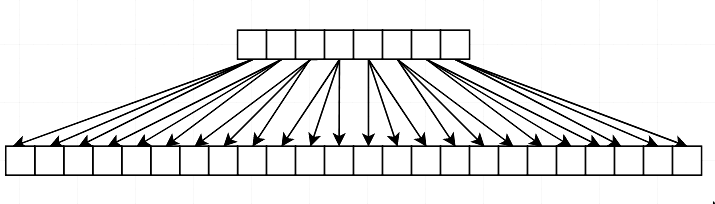
\includegraphics[scale= 0.25]{Potrajanie/potrajanie_proste.png}\\
Możliwe jest rozwinięcie kodu o przeplot danych.
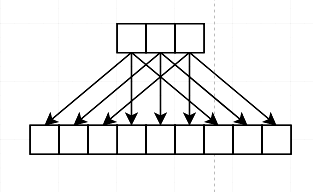
\includegraphics[scale=0.25]{Potrajanie/potrajanie_przeplot.png}

\end{center}

\end{frame}

\subsection{BCH}
\begin{frame}{BCH}
Nazwa pochodzi od nazwisk autorów kodu, Hocquenghema, który skonstruował kod w roku 1959 oraz niezależnych od niego badaczy Bose i Chaudhuri z roku kolejnego.\\
Kodowanie Bose–Chaudhuri–Hocquenghema
Parametry:\\
• długość wektora kodowego $n=2m–1$\\
• liczba pozycji kontrolnych $n-k ≤ mt$\\
• min. odległość Hamminga $d_{Hmin}≥2t+1$\\
Kod koryguje do t błędów\\
Kody Hamming są podzbiorem kodów BCH
(BCH z t=1 jest kodem Hamminga)
stosowane powszechnie w praktyce;
wielopoziomowe;
cykliczne;
o zmiennej długości;
służące do korekcji błędów losowych (w przybliżeniu do 25% całkowitej liczby cyfr);
binarne bądź używane z modulacją PSK (phase-shift keying), jednak największe znaczenie mają w praktyce kody binarne;
mają strukturę algebraiczną;
ich metody konstrukcji o zadanych właściwościach są stosunkowo proste i efektywne;
konstrukcja ich koderów i dekoderów prostsza w porównaniu z innymi kodami;

Kody BCH należą do kodów cyklicznych, czyli kodów wielomianowych o długości słowa kodowego \emph{n}, których wielomian generujący \emph{g(x)} (niezbędny do konstrukcji słowa kodowego) jest dzielnikiem wielomianu. Można udowodnić, że istnieje taki wielomian k(x) stopnia k, że:
g(x)k(x)=x^n+1 lub (x^n+1)modg(x)=0.

Dla m nal.do Z i t<2^{m-1} istnieje kod BCH o n = 2^m-1. Może korygować do t błędów i ma nie więcej niż mt elementów kontrolnych.

Parametry:
n=2^m-1
k>=2t+1
d_min>=2t+1

\end{frame}

%\subsubsection{Kod Haminga}
%\begin{frame}{Kod Haminga}
%Przykład kodowania i dekodowania danych w kodzie Haminga
%\begin{center}
%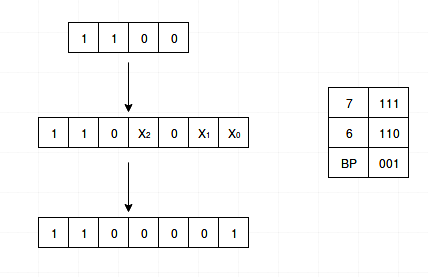
\includegraphics[scale= 0.30]{Haming/Kodowanie_Haming.png}
%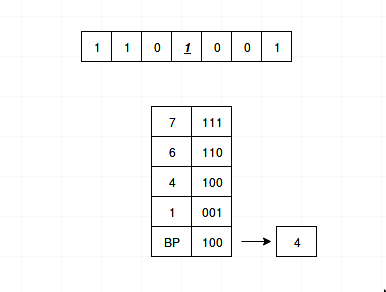
\includegraphics[scale=0.30]{Haming/Dekodowanie_Haming.png}
%\end{center}
%\end{frame}

\section{Kod Hamminga}
\begin{frame}
\centering

\includegraphics[scale= 0.5]{image_source/ham.jpg}
\end{frame}

\section{Kodowanie Reeda-Salomona}
\begin{frame}{Kodowanie Reeda-Salomona}
Niebinarna wersja kodów BCH.\\
Zastosowanie: systemy DVB-T, DVB-H, WiMAX\\
	\begin{flushright}
    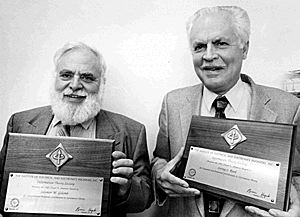
\includegraphics[scale= 0.5]{image_source/ReedSolomon.jpg}
    \caption{Irving S. Reed i  Gustave Solomon}
    \end{flushright}
\end{wrapfigure}
\end{frame}

\section{Porównanie}
\begin{frame}{Porównanie}
\centering
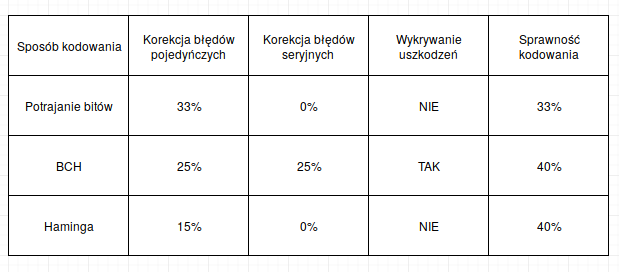
\includegraphics[scale= 0.5]{image_source/porownanie.png}
%\begin{itemize}
%		\item blokowe, czy jest przeplot
%		\item sprawność (współczynnik) kodowania k/n
%		\item możliwości detekcyjne i korekcyjne, dmin?
%		\item systematyczne czy niesystematyczne?
%		\item binarny/niebinarny???
%		\item zysk kodowy w dB???
%		\item odporność na błędy seryjne
%		\item \ldots
%\end{itemize}
		
\end{frame}

\section{Bibliografia}
\begin{frame}{Bibliografia}
	
\end{frame}

\section*{Pytania}
\begin{frame}
	\centering \Large\emph{Dziękujemy za uwagę. Pytania?}
\end{frame}

\end{document}